\section{Anwendungsfälle}
% [ ] Präsentieren sie einen sinnvollen Anwendungsfall in dem ein bestimmter Fakt, ein Muster oder die Abwesenheit eines Musters visuell festgestellt wird.
% [ ] Begründen sie warum dieser Anwendungsfall wichtig für die Zielgruppe der Anwenderinnen ist.
% [ ] Diskutieren sie weiterhin, ob die oben beschriebene Information auch mit anderen Visualisierungstechniken hätte gefunden werden können.
% [ ] Falls dies möglich wäre, vergleichen sie die den Aufwand und die Schwierigkeiten ihres Ansatzes und der Alternativen. 
Nachdem die Anwendungsaufgaben formuliert und die Visualisierungen abgeleitet wurden, werden nun drei Anwendungsfälle vorgestellt, bei deren Bearbeitung der Anwender durch die Visualisierung unterstützt wird.

\subsection{Anwendung Visualisierung Eins}
% Präsentieren sie einen sinnvollen Anwendungsfall
Die Vereinigten Staaten belegen mit 40 Goldmedaillen und insgesamt 126 Medaillen den ersten Platz im Medaillenspiegel der Olympischen Sommerspielen 2024. Bei diesem Ergebnis ist es naheliegend von der sportlich erfolgreichsten Nation zu sprechen. Schließlich wurden $12,7\%$ aller Olympischen Medaillen von US-Athleten gewonnen. Durch Klick auf den entsprechenden Eintrag im Medaillenspiegel wird dem Anwender die Verteilung der Medaillen für die Vereinigten Staaten im SunBurst-Diagramm geladen, wie in \autoref{fig:usa} dargestellt.
\begin{figure}[!tb]
    \centering
    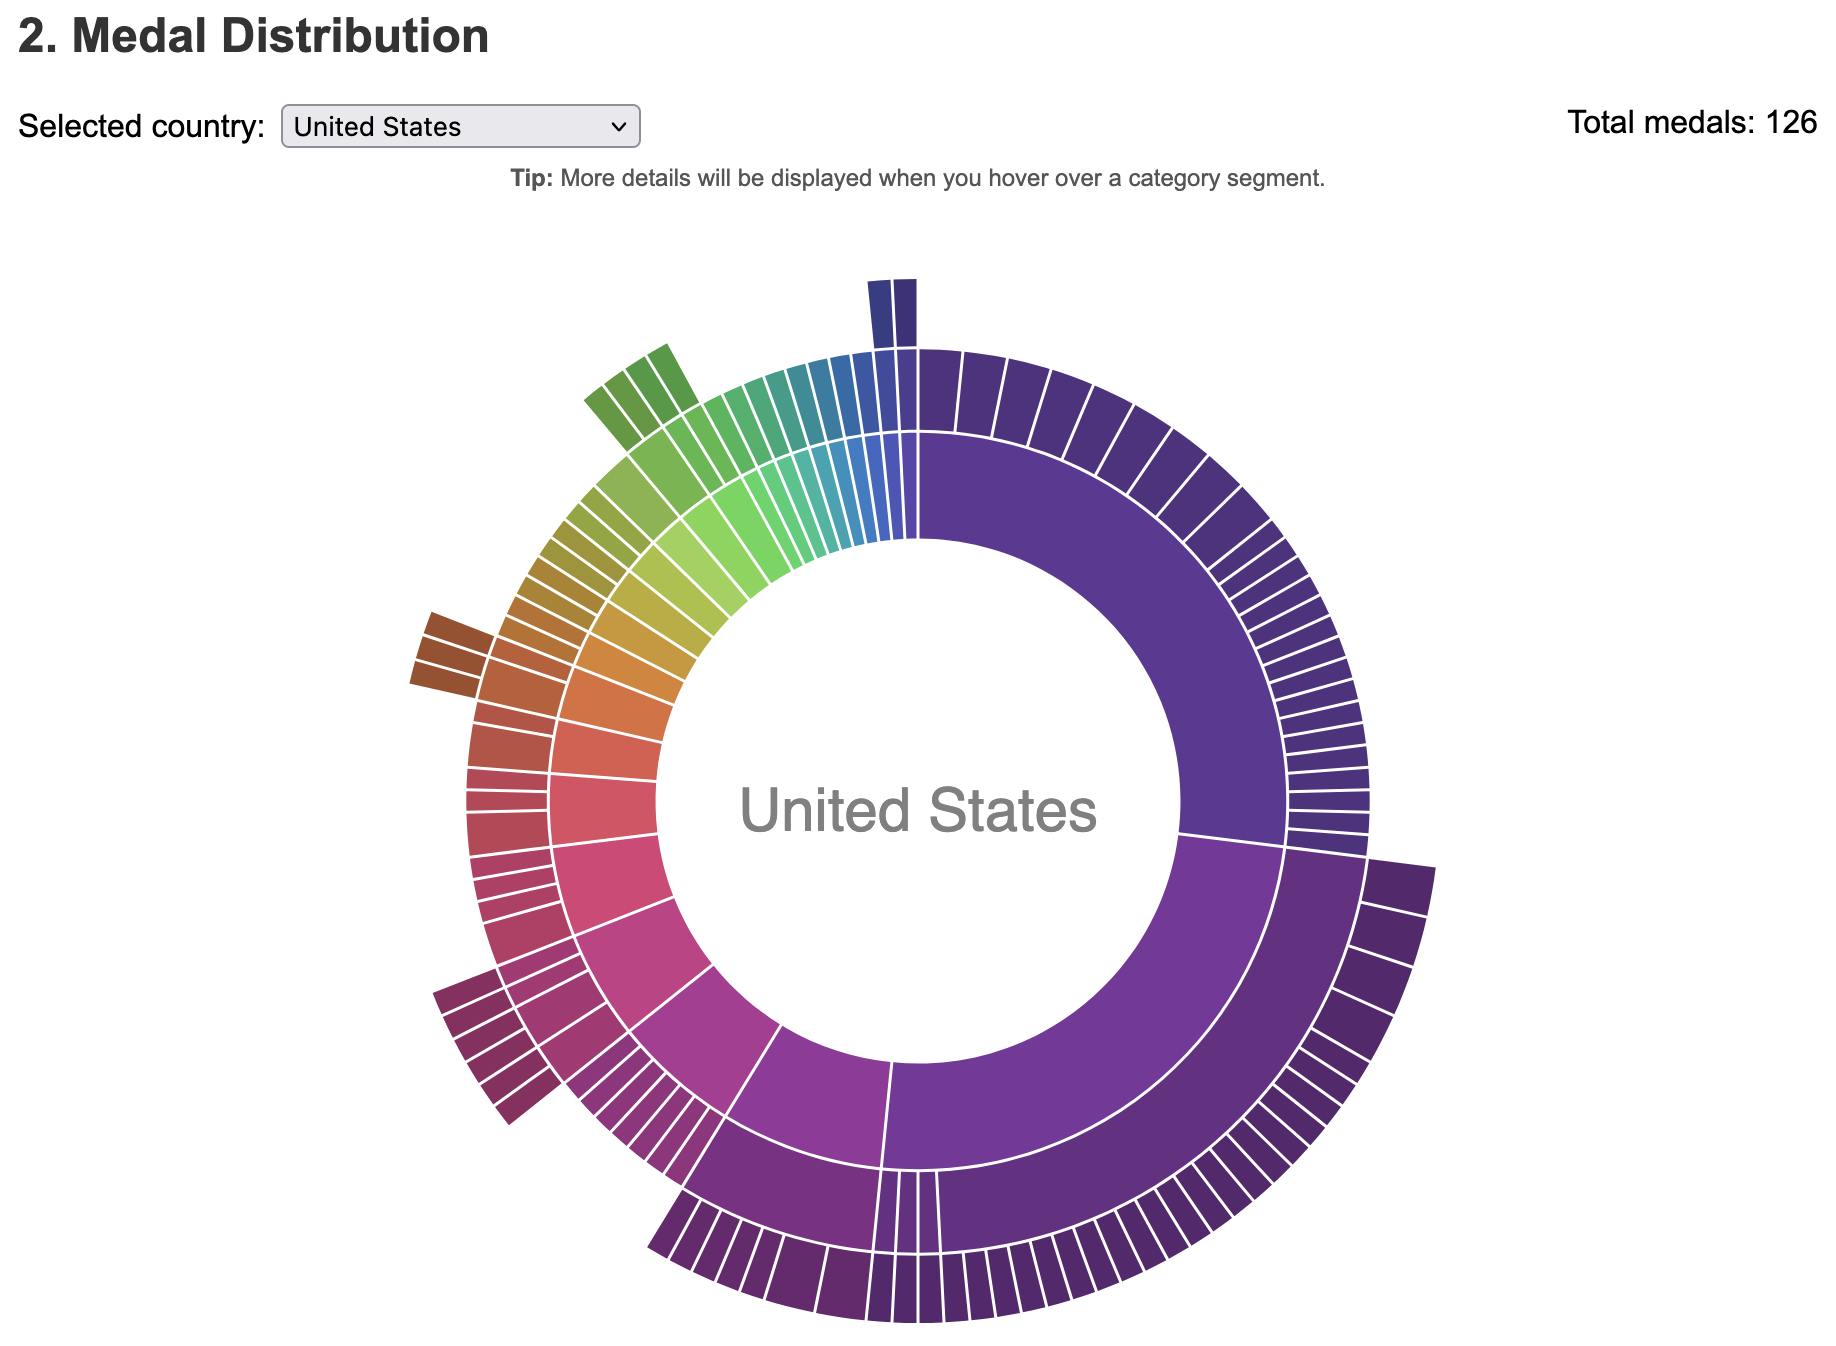
\includegraphics[width=0.5\linewidth]{img/SunBurst_USA.png}
    \caption{Medaillenverteilung der Vereinigten Staaten}
    \label{fig:usa}
\end{figure}

Auf den ersten Blick fällt das Diagramm durch seine vielen Farben auf. Vor allem oben links sind viele verschiedene Farben sichtbar, welche unterschiedliche Sportarten repräsentieren. Das bedeutet, dass die Vereinigten Staaten in vielen unterschiedlichen Sportarten Medaillen gewinnen konnten. Bei genauerer Betrachtung können 26 verschiedenen Sportarten gezählt werden. Weiterhin fällt das Diagramm auf der rechten Seite durch viele violette Farben auf. Große Flächen gleicher Farbe bedeuten, dass ein großer Anteil der Medaillen in der gleichen Sportart gewonnen wurde. Per \textit{Mouse-Hover} über die Kreissegmente werden $26.98\%$ der Medaillen der Kategorie \textit{Athletics} und $24,6\%$ der Kategorie \textit{Aquatics} zugeordnet. Somit stammen $50\%$, also 63 Medaillen, nur allein aus diesen beiden Sportarten. 

% Begründen sie warum Anwendungsfall wichtig für Zielgruppe ist
Die Interpretation dieser Ergebnisse kann je nach Anwender sehr unterschiedlich ausfallen. Da China im Medaillenspiegel Platz zwei hinter den Vereinigten Staaten belegt hat, könnte ein chinesischer Reporter Nachforschungen zu diesem Ergebnis anstellen. Anhand des Medaillenspiegels kann er nur erkennen, dass die Vereinigten Staaten mehr Medaillen gewonnen haben als China und somit sportlich erfolgreicher waren. Mithilfe der Visualisierung kann er aber die Verteilung der Medaillen nach Sportarten und Disziplinen betrachten und argumentieren, dass die Vereinigten Staaten ohne die erfolgreichen Sportler in den Kategorien \textit{Athletics} und \textit{Aquatics} nicht besser als China gewesen wären. Ein Schwimmer könnte das Ergebnis ganz anders interpretieren und würde aufgrund der Dominanz der Vereinigten Staaten in seiner Sportart mit dem Gedanken spielen, sein Training in dieses Land zu verlagern, um von den offensichtlich guten Voraussetzungen zu profitieren. In beiden Fällen hätte ihnen der Medaillenspiegel nicht ausgereicht, um diese Informationen zu erhalten. Erst durch die Visualisierung konnten sie diese Analyse durchführen.

% Diskutieren sie wo Information auch mit anderen hätte gefunden werden
Als Alternative zu dem SunBurst-Diagramm wurden bereits TreeMaps genannt. Diese Visualisierungstechnik kann die Verteilung der Medaillen nach Sportarten und Disziplinen ebenfalls darstellen. Dabei würde die Hierarchie durch ineinander geschachtelte Rechtecke abgebildet werden. Die Farben könnte in gleicher Weise eingesetzt werden. Der wesentliche Unterschied ist die Art der Darstellung der Hierarchie, bei der in der TreeMap ineinander geschachtelten Rechtecke und im SunBurst-Diagramm konzentrische Ringsegmente  als zusammengehörig interpretiert werden müssen. Die meisten Anwender werden Kreis- bzw. SunBurst-Diagrammen schon häufig in ihrem Alltag begegnet sein, sodass diese für sie einfacher zu interpretieren sind als TreeMaps. Der technische Aufwand für die Implementierung dürfte bei beide Visualisierungen ähnlich groß sein.

\subsection{Anwendung Visualisierung Zwei}
% Präsentieren sie einen sinnvollen Anwendungsfall
Der kleine Inselstaat Grenada erzielte bei den Olympischen Sommerspielen 2024 mit zwei Bronzemedaillen das beste Ergebnis in der Geschichte. Aus diesem Grund dürfte die Freude darüber sehr groß gewesen sein. In dem Medaillenspiegel belegt es aber nur Platz 81, da bei diesem Ranking externe Einflussfaktoren, wie zum Beispiel die geringe Einwohnerzahl von gerade einmal $117.000$ Einwohner, nicht in die Bewertung einfließen. Aber aus dieser Perspektive sind zwei Medaillen eine enorme Leistung. Daher sollen die Anwender die gewonnen Medaillen mit demografischen und wirtschaftlichen Einflussfaktoren in Beziehung setzen und die Frage nach der sportlich erfolgreichsten Nation mithilfe dieser alternativen Länderrankings neu beantworten. Die in \autoref{fig:grenada} dargestellte Visualisierung zeigt den Vergleich der Platzierungen von Grenada in den verschiedenen Länderrankings. Dabei wird deutlich, dass Grenada sowohl im Vergleich \enquote{Medaillen pro Einwohnerzahl}, als auch \enquote{Medaillen pro Bruttoinlandsprodukt} zu den erfolgreichsten Ländern gehört. Außerdem können im Hintergrund viele sich kreuzende Linien beobachtet werden. Das bedeutet, dass Länder die im Medaillenspiegel einen guten Platz belegt haben, unter dem Einfluss externer Faktoren nicht mehr so gut bewertet werden. Umgedreht schneiden Länder mit einer schlechten Platzierung im Medaillenspiegel besonders gut in den alternativen Länderrankings ab.

\begin{figure}[!tb]
    \centering
    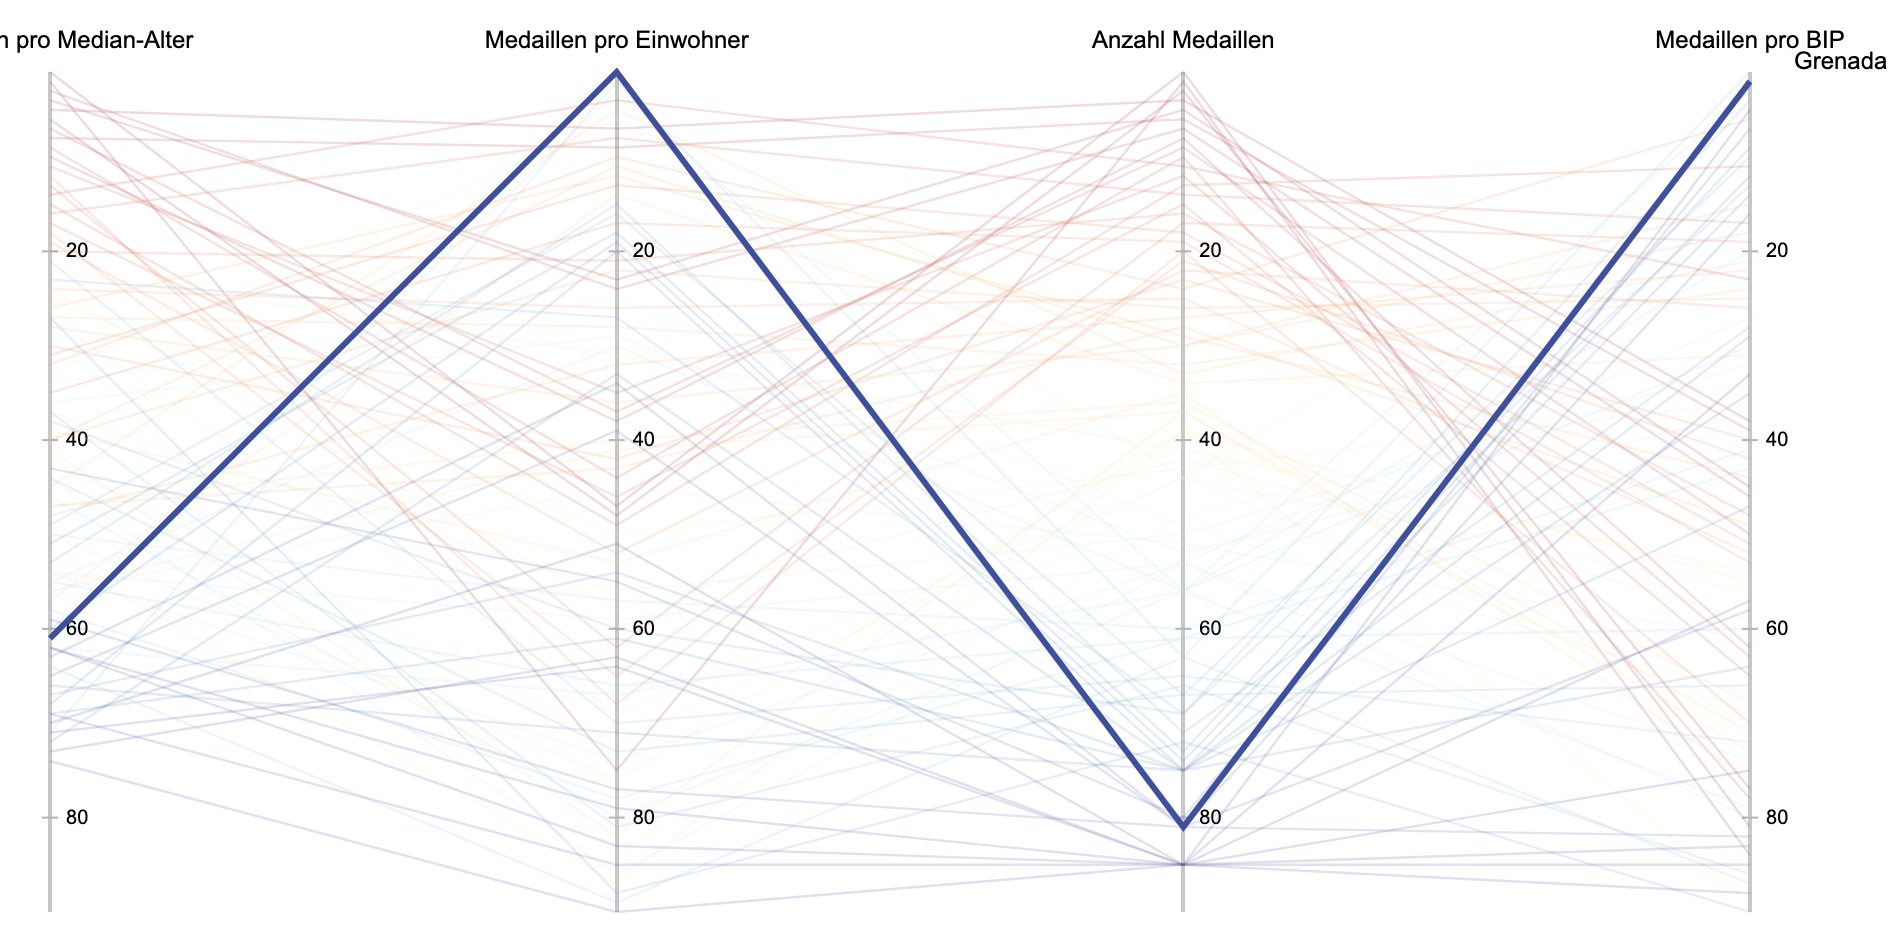
\includegraphics[width=0.5\linewidth]{img/Grenada.png}
    \caption{Grenada in den verschiedenen Länderrankings}
    \label{fig:grenada}
\end{figure}

% Begründen sie warum Anwendungsfall wichtig für Zielgruppe ist
Der bekannte Medaillenspiegel bewertet nur die absolute Anzahl gewonnener Medaillen, wo Grenada mit zwei Medaillen nur einen der hinteren Plätze belegt. Unter diesen Umständen würde niemand Grenada als das sportlich erfolgreichste Land der Olympischen Sommerspiele bezeichnen. Die demografischen und wirtschaftlichen Entwicklungen sind in diesem Land aber ganz anders als zum Beispiel in den Vereinigten Staaten. Aufgrund des viel geringeren Bruttoinlandsprodukt stehen dem Land auch viel weniger finanzielle Mittel für den Sport zur Verfügung. Indem demografische und wirtschaftliche Einflussfaktoren in die Bewertung aufgenommen werden, wird dem sportlichen Erfolg Grenadas mehr Bedeutung gegeben. Dadurch können die Anwender die sportlichen Erfolge einer Nation aus einem anderen Blickwinkel betrachten und die Frage nach der sportlich erfolgreichsten Nation neu beantworten.

% Diskutieren sie wo Information auch mit anderen hätte gefunden werden
In dem beschriebenem Anwendungsfall werden die verschiedenen Länderrankings für ein konkretes Land miteinander verglichen. Dies könnte auch mit einem Scatterplot umgesetzt werden. Jedoch ist die Anordnung der Länderrankings entlang der Achse fest und kann nicht beliebig vertauscht werden. Dadurch ist ein direkter Vergleich von zwei Länderrankings nicht möglich. Die Anordnung der Achsen in den Parallelen Koordinatensystem ist aufgrund des Aufbaus dieser Visualisierung ohne Probleme möglich. Darüber hinaus wurden die sich kreuzenden Linien in der Grafik angesprochen, wodurch allgemeine Änderungen in der Platzierung schnell erkannt werden können. Diese Information kann mit anderen Visualisierungstechniken nicht besser dargestellt werden, als in der kompakten Form in dem Parallelen Koordinatensystem. 

\subsection{Anwendung Visualisierung Drei}
% Präsentieren sie einen sinnvollen Anwendungsfall
Bei der Betrachten des historischen Medaillenspiegels in \autoref{fig:allTime}, sortiert nach dem Kriterium \enquote{All-Time}, können bei dem direkten Vergleich von Polen und Finnland interessante Entwicklungen beobachtet werden. Bei der Darstellung der Medaillenspiegel von Polen fällt eine Reihe gleichfarbiger Zellen ab dem Jahr 1984 auf. Diese sind in orange einfärbt und stellen bei einem Blick auf die Legende zwischen 10 und 19 Medaillen pro Olympiade dar. In der darunterliegenden Zeile sind die Medaillenspiegel von Finnland dargestellt. Dort ist ein dunkler Bereich in den Jahren von 1912 bis 1952. Ab dann werden die Zellen immer heller und im Jahre 2024 ist die Zelle komplett weiß, was bedeutet, dass Finnland bei der letzten Olympiade keine Medaille gewonnen hat.

\begin{figure}[!tb]
    \centering
    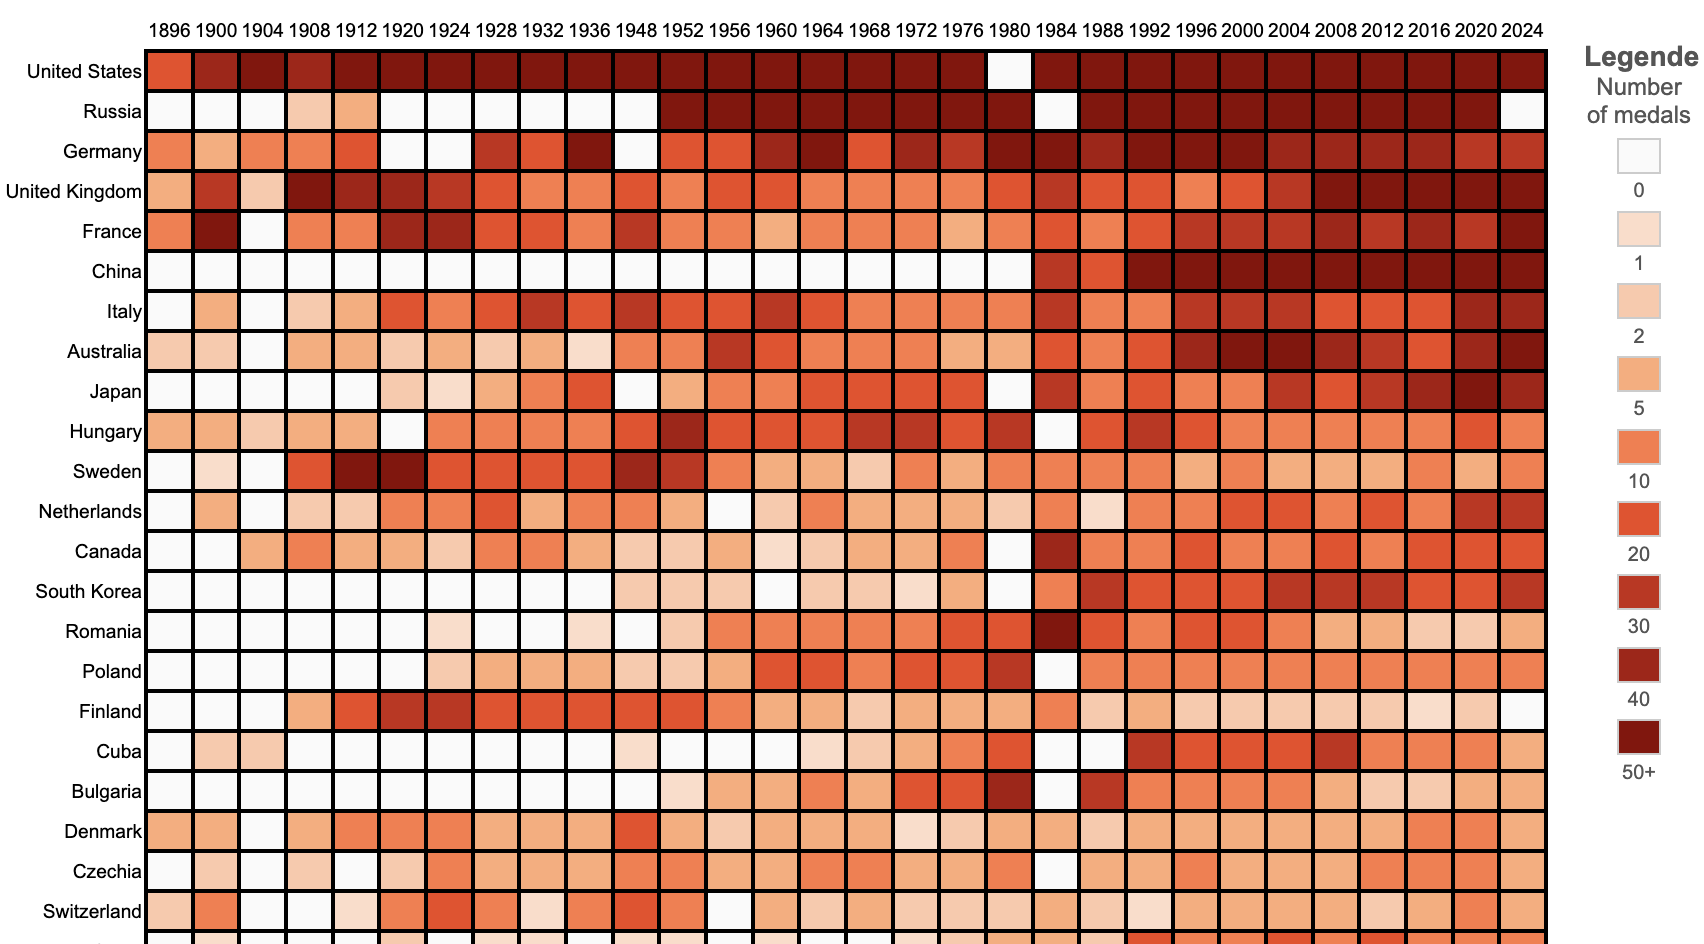
\includegraphics[width=0.65\linewidth]{img/AllTime.png}
    \caption{Historischer Medaillenspiegel}
    \label{fig:allTime}
\end{figure}
% Begründen sie warum Anwendungsfall wichtig für Zielgruppe ist
Die Beobachtung von Polen zeigt, dass dieses Land regelmäßig neue Medaillengewinner beglückwünschen kann und offensichtlich eine gute Talententwicklung hat. Zudem ist davon auszugehen, dass Polen diesen Trend fortsetzen kann und auch bei der nächsten Olympiade Medaillen gewinnen wird. Diese Erkenntnis ist für Sponsoren sehr wichtig, denn diese möchten Sportler und Länder fördern, die gute Aussichten auf Medaillen haben. Anders sieht es für Finnland aus. Dieses Land konnte zum ersten Mal seit 100 Jahren keine Medaille gewinnen. Während andere Länder, wie zum Beispiel Estland, auch keine Medaillen gewonnen haben, war dieses Ereignis bei einem Blick auf die historische Entwicklung von Finnland aber vorhersehbar. Seit 1952 werden die Farben in den Zellen von Finnland immer heller, was eine immer geringere Anzahl an Medaillen bedeutet. Dieses Information ist für Sportler, wie auch Sponsoren sehr wichtig, um sich frühzeitig nach Alternativen umzusehen.

% Diskutieren sie wo Information auch mit anderen hätte gefunden werden
Der historische Medaillenspiegel aller Länder umfasst sehr viele Daten. Um diese auszuwerten und zu analysieren hat sich die HeatMap als optimal erwiesen, da die vielen Informationen sehr kompakt und übersichtlich dargestellt werden können. Die Entwicklungen eines Landes können durch ScatterPlots oder Säulendiagramme visualisiert werden, jedoch können diese Visualisierungen nicht die Entwicklungen aller Länder gleichzeitig darstellen. Die Grafiken wären überladen mit Informationen und sehr unübersichtlich. Ein weiterer Vorteil der HeatMap ergibt sich aus der Kodierung der Werte auf Farbe. Die Farbänderungen sind nach dem Konzept der \textit{Preattentive Recognition} \cite{preAttent} sehr schnell und unterbewusst wahrnehmbar. Deshalb fällt im Beispiel von Polen die lange Reihe gleicher Farbwerte und bei Finnland die immer heller werdenden Zellen sofort auf. Dieser Eigenschaft der Wahrnehmung lässt sich mithilfe der HeatMap am besten ausnutzen.